\documentclass[12pt,a4paper]{article}
\usepackage[latin1]{inputenc}
\usepackage{amsmath}
\usepackage[T1]{fontenc}
\usepackage{palatino}
\usepackage{algorithm2e}
\usepackage{algorithmic}
\usepackage{hyperref}
\usepackage{amssymb}
\usepackage{graphicx}
\author{Alexandros-Panagiotis Oikonomou}
\setlength{\parindent}{15pt}
\begin{document}
\begin{titlepage}
\begin{center}
\begin{LARGE}
Electronics and Computer Science
Faculty of Physical and Applied Sciences
University of Southampton 
\end{LARGE}
\\[2cm]
\begin{large}
Alexandros-Pana Oikonomou
\\
1$^{st}$ May 2013
\\[2cm]
Solving the Conjugate Gradient Method in a SpiNNaker Machine
\\[3.5cm]
Project Supervisor: Jeff Reeve
\\Second Examiner: Marcus Breede
\\[3.5cm]
A project report submitted for the award of
\\BSc Computer Science
\end{large}
\end{center}
\end{titlepage}
\section*{Abstract}
\pagenumbering{gobble}
SpiNNaker is an asynchronous, event-driven parallel architecture designed to simulate
the human brain. It has been designed to operate as a large scale neural network in
real-time using a System-on-Chip multi core system. Its architecture is different from
usual parallel computers, since cores use spikes to communicate with each other. That
way usual pitfalls of parallel computing, such as race conditions and deadlocks are
avoided. So far the most prominent uses of this architecture have been in
neuroscience and robotics. The aim of this project is to put into use SpiNNaker's
architecture and bring it closer to classic computer science problems, while solving
them optimally. The algorithm to solve in this project is the conjugate gradient
method, an iterative way of solving systems linear equations. The algorithm successfully runs on the simulator and reduces the time complexity of the most expensive operations of the algorithm.
\newpage
\tableofcontents
\newpage
\section*{Acknowledgments and Statement of Originality}
I would like to thank my supervisor Jeff Reeve for his help and support throughout this project, as well as providing inspiration for the topic.
\newpage
\section{Introduction}
\pagenumbering{arabic}
\subsection{Aim}
The aim of this project is to correctly solve the Conjugate Gradient Method\cite{hestenes1952methods} on a SpiNNaker chip, thus using the massive parallelism that this machine provides to reduce the time complexity of the aforementioned algorithm. This is accomplished by reducing the time complexity of the most expensive operations of the algorithm which are matrix-vector multiplication and the scalar product of vectors. The complexity is reduced dramatically, due to the abundant number of cores provided from the architecture. This report provides a detailed analysis of this project and its constitutes, the background research done to launch this project, along with design and implementation choices.
\subsection{Reasons and Justification}
\indent
SpiNNaker is an architecture inspired by the biology of the human brain. Its optimal configuration has over a million cores\cite{navaridas2009understanding}, which have mainly been used to simulate the neurons of the human brain and in some cases, robotics.

However little work had been done into putting the SpiNNaker architecture to solve classic computer science problems. That is why a problem such as the Conjugate Gradient Method had been proposed, which is a very common solution to optimization problems. In addition to that, the SpiNNaker architecture offers new parallel programming paradigms, that escape some common parallel programming pitfalls such as race conditions, deadlocks, mutual exclusion etc\cite{sharp2011event}.
\subsection{Overview}
This report starts off by giving a detailed analysis of the SpiNNaker architecture and its constitutes, and the Conjugate Gradient Method.It continues by outlining the design and the tools used to solve the given problem and provides an in-depth examination of the implementation issues and solutions. It ends with a critical evaluation and conclusion.
\newpage
\section{Background}
\subsection{The neuron}
To make the explanation of the SpiNNaker architecture smoother, the design from which the SpiNNaker chip was inspired will be outlined. This is no other than the human neuron.

The human neuron is an electrically excitable cell that processes and transmits information through electrical and chemical signals. Its basic costitutes are the the soma, the dendrites and the axon. The soma is the body of the neuron. A dendrite receives signals from the soma of the neuron that it belongs to, or other neurons. The dendrite extends for hundreds of micrometers and branches multiple times, thus forming a dendritic tree, which connects with other neurons axons. The axon is used to transmit signals to other neurons and it extends from the soma of the neuron to a dendrite. All human neurons have only one axon. Given the above analysis the dendrites could be described as the inputs of a neuron
\\[0.5cm]
\begin{figure}[h!]
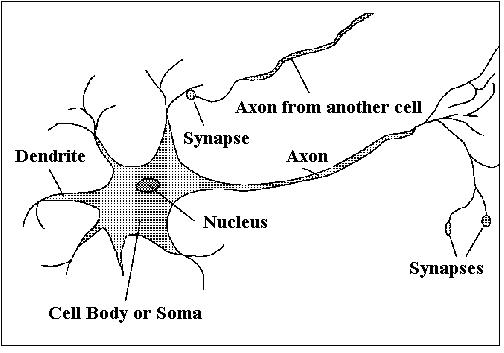
\includegraphics[width=300pt,height=200pt,scale=2]{Pics/neuron.jpg}
\centering
\caption{A neuron}
\end{figure}

One of the most important parts of the neuron structure is the synapse. The synapse is where the contact happens between the axon of a neuron and the dendrite or the soma of another. It is where information from one neuron is transmitted to the other. When a set of neurons are connected with each other through synapses, then they create a neural network.

Finally, the communication between neurons is accomplihed through spikes, which are either chemichal or electrical\cite{gerstner2002spiking}.

Given the terms in this section, the name of the SpiNNaker chip is deductable. It stands for Spi(king)N(eural)N(etwork) architecture.
\subsection{The SpiNNaker architecture}
As mentioned before the SpiNNaker architecture is inspired by the biology of the brain, and more specifically, neurons. However, its architecture is not constrained by the biology of the brain, but many techniques to speed up computation are used. It differs from other supercomputers, which  usually have a lot of strong processors with slow network capabilities. The design of the architecture was made with two concerns as its main priority. The first one being MIPS(millions of instructions per-second) per mm$^2$. Namely how many instructions can be performed in an area of silicon. The second one was MIPS per watt, which means how many instructions per second can be performed given a fixed amount of energy. Its most optimal configuration will use a million cores and will be able to simulate over a billion neurons\cite{furber2007neural}.
\subsubsection {SpiNNaker chip Overview}
The heart of the SpiNNaker architecture is the SpiNNaker chip. Its main components are 18 identical ARM cores that run at around 100Mhz each, a router, a system NoC(Network-on-Chip) which connects to the router of the chip and a 128 MB SDRAM. At startup, in each chip a processor is selected to act as a Monitor processor, with the task of performing the management of the given chip's system. The remaining ARM cores perform the calculations for the given problem, with the exception of one which is reserved as a spare. The spare processor exists for the emergency of another core having a malfunction\cite{furber2007neural}. Each core has the ability to hold 32KB of instructions and 64KB of data. Since this is not enough space, all other data is saved in the SDRAM which can hold up to 1GB of data\cite{navaridas2009understanding}.
\begin{figure}[h!]
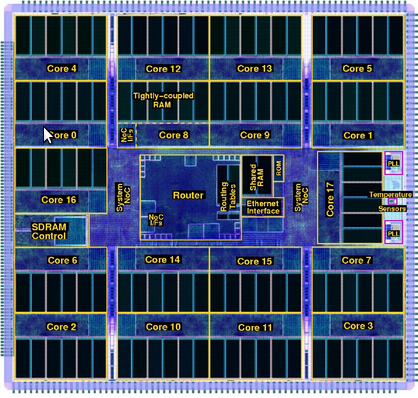
\includegraphics[width=250pt,height=150pt,scale=2]{Pics/chip.png}
\centering
\caption{The SpiNNaker chip\cite{spinnweb}}
\end{figure}
\subsubsection{The router}
As mentioned before the architecture supports low-delay communication, with less powerful processors, than those used in most supercomputers. To accomplish that, the system uses asynchronous multicast packets to communicate between cores. This is done through the router which lies in each chip.

The router exists as the part of the NoC and its primary role is to direct packets that arrive and packets that are sent or need to be forwarded. The router has 20 ports for the ARM cores that are located in the given chip and is able to forward one packet at a time. The router works faster than a transmission port, which results into the router being most of the time lightly used. It is designed to support point-to-point communication, using small packets. The use of multicast packets helps to reduce the amount of packets that exist in the network at any given moment. To even further enhance the quickness of the network, the architecture supports default routing. This means that not all connections need to exist in the routing tables, in order to have the packets forwarded to their eventual diestination. This concept will be explained in more depth in the next section.

The functionality of the router is pretty simple. When a packet arrives from the input port, then the router will try to send it to an output port. If there is a problem during transmission, then the router will keep trying to send it and after a while it will try the emergency route(also explained in the next section). If the emergency route still does not work and a certain amount of time has passed, then the packet will be dropped. To implement this, the time of delivery of a packet is stored in the header of each packet.

\begin{figure}[h!]
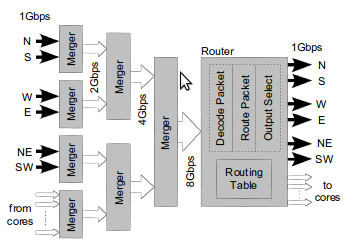
\includegraphics[width=250pt,height=150pt,scale=2]{Pics/router.png}
\centering
\caption{The router\cite{navaridas2009understanding}}
\end{figure}
To further understand this concept, the topology of the system needs to be considered.
\subsubsection{Topology}
In order to have a million cores available for processing a number of SpiNNaker chips need to be connected and work efficiently as a whole. To reach that goal an effective topology is important.
\begin{figure}[h!]
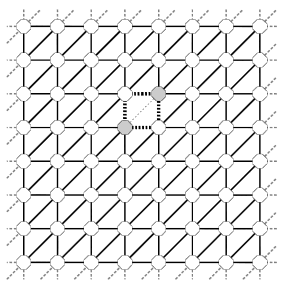
\includegraphics[width=250pt,height=250pt,scale=2]{Pics/topology.png}
\centering
\caption{
\emph{The SpiNNaker topology\cite{navaridas2009understanding}. This is an example of what an 8x8 would look like.Each circle is a SpiNNake chip and the lines between them are the connectivity.}}
\end{figure}
\vspace{20pt}
Considering Figure 4, it is visible that the topology is viewed by the system as a 2D mesh, with chips having a fixed amount of neighbours and specific base connections. Any chip is able to communicate directly to 6 other chips. This is also depicted in Figure 3, where the positions of these chips are shown. In general each chip can directly communicate with chips that are located North, South, West, East ,NorthEast, and Southwest of its respective position. This however does not apply for chips that are in the perimeter of the mesh, since in some of the positions described above, some neighbouring chips will not exist\cite{furber2012overview}. 

Returning now to the default routing mentioned in the previous section, if a packet arrives to a router, and the router does not have an entry for it, a then it will be forwarded to the chip opposite to the one it came from. For example, if a packet comes from the East and the aforementioned condition is met, then it will be forwarded to the West. This helps reduce the size of the routing tables in each chip\cite{khan2008spinnaker}.

In addition to the default routing, the topology also provides for two-hop routes among neighbor chips, as shown in Figure 4. These routes are named emergency routes and their functionality is to bypass any faulty connections that might exist between connections\cite{navaridas2009understanding}\cite{plana2007gals}.

\subsubsection{Packets}
The packets used in the architecture are all multicast packets. They are asynchronous and relatively small. Having multicast packets means that one packet might have many different destinations, and with potentially a million cores, they can have thousands of destinations. For that reason, the packets do not contain the destination(s) they are supposed to reach, but rather only the source. Their size is of around 40 or 70 bits and their transmission is done completely by the hardware of the system, thus achieving high bandwidth\cite{spinnweb}\cite{navaridas2009understanding}. It is also notable that, when simulating a billion neurons, unique addresses are needed to acknowledge them. Hence 32-bit addresses are used to represent items in the cores. In this architecture, the main packets used can be divided in two types.
\begin{itemize}
\item Multicast packets(Type 0). Consists of 32-bit source address, 8 bits of control and 32-bit payload. These types of packets are delivered to processors and usually would contain information for computation
\item Point-to-point packets(Type 1). Consists of 16-bit source \emph{chip} address, 16-bit target \emph{chip} address, 8-bit control payload and 32-bit payload. It is a command/control packet and is used when the Monitor Processor communicates with the target chip\cite{docfile}
\end{itemize}

In this project Type 0 packets have mainly been used.
\subsubsection{Routing Tables}
A mention of the routing tables is also important in understanding the architecture. Optimally, one would want for all cores to communicate with all the other cores in the system. However, that would be impractical, since the data structure to hold the entries for the routing table would have to be enormous.

This architecture supports routing tables of 1024 entries. Each entry is of 32-bit size, since it needs to hold addresses for the routing. The nature of the most siginificant bit of the source determines if a particular packet is for distributing locally to the cores, or if it should be linked and forwarded to other chips\cite{docfile}.
\subsubsection{Bandwidth}
Having discussed the architecture and its network, a mention of the bandwidth bisection that is offered will be outlined here. Assuming the optimal configuration of the SpiNNaker architecture with a million cores, then it is safe to assume that the number of chips that will be used, would be around 63K. If we would split the topology in two then the optimal goal would be to have all the neurons of one half connected to at least one neuron in the other half. That way, the bandwidth in the border would be 6.4G packets/sec. Another safe assumption is that the 2D mesh for this machine would be 256x256. Given that each node should carry 25M packets. This would offer more possible connections and would achieve more and faster results.\cite{docfile}\cite{navaridas2009understanding}.
\newpage
\subsection{Software}
There is a lot that comes when trying to run any kind of software in a SpiNNaker board. The basic devices that are used to run software are three.
\begin{itemize}
\item Host Machine, which is mainly used for input and output, and it is the component that the user interacts with to start an application
\item Monitor Cores. This is the same Monitor core that was discussed previously. Its main use is monitoring and managing the system and the application cores. One of them also communicates with the host, in order to start up the program.
\item Application Cores, which are used to carry out the computation of the application.\cite{furber2012overview}
\end{itemize}

At this point it is noteworthy to mention that the programming model of the machine is event-driven, meaning computations occur when specific events take place. More on that will be covered in later sections
\subsubsection{Startup}
In order to do the startup and interact with the aforementioned devices some kind of software needs to be used. For the Host machine to interact with the main Monitor Core \emph{ybug} is used. It is also used to start applications. Ofcourse ybug does not communicate only with the hardware of the monitor core. There is another software called \emph{scamp}, that works on top of the Monitor Core. It interacts with the ybug and the \emph{sark}, which is a software that is used by the application cores. Sark lets the user to manipulate some hardware parts of a SpiNNaker chip.\cite{spinnweb}
\subsubsection{Local Data Structures}
Before the application starts running, startup applications need to be run first. These include finding the state of the machine, finding a communications tree for the cores and chips and sketching out the point-to-point tables.

\paragraph{The state of the machine}
To discover the state of the machine, each chip checks its cores and the connections between them to check whether any broken links exist. The algorithm starts by selecting a root node and marking it with a Request(R) token. Each time a core has an R token it sends an Acknowledge(A) label to all the incoming ports. If the labeling is successful, then that incoming port is deemed Good. Otherwise it tries to send an R token to that port and it marks it as Broken\cite{jefflec}.
\paragraph{Building a communications tree}
In order to build a communication tree a breadth first tree traversal is used. To achieve that, a root node is selected and given the token Forward(F) at first. The root node speaks to neighbouring nodes and after giving them the label Child it says to them to also send F tokens to all their neighbours, thus making them both a Parent and a Child. Once there are not any more unlabelled nodes, the nodes are instructed to return a Backwards(B) token to their parent nodes. That way the system becomes aware of which nodes communicate with each other. If by any chance two nodes send to each other a B token through the same port, then that port is deemed non communicational and is labelled Unused. The reason for that is to avoid any loops in the system\cite{jefflec}.
\paragraph{Creating the P2P Tables}
Nodes need ID's in order to have packets sent correctly to certain destinations. Point-to-Point tables are used to list the ID's of nodes, so the packets know which ports they should follow. At first all nodes are undefined(U). If we were to find the entry for one undefined node then the table would mark its own incoming port and send its port to all other ports.  That way all the other chips in the board would know what port to use to communicate with that node. For the nodes that are on the same chip with that node............If that is done for the all of the nodes in the system, then the P2P table is built\cite{jefflec}. 

\subsubsection{Program Loading}
In order to begin running a program some input needs to be provided to the system. The way this is currently done is by using the static model. With the static model the network topology, the connections between nodes and the allocation of the hardware is provided explicitely and externally by the user, before the execution of the program. Moreover, data and additional execution information needs to be defined before the program is loaded in the machine. This information is read from an external machine and written again in a fashion that is readable by the machine in the form of binary files. The Host starts the execution of the program, after the 'readable' version has been loaded to the machine. When the program terminates, or the user wishes to terminate it, then the Host issues a halt command to stop all operations\cite{docfile}.

There is an additional model for loading data in the system called the dynamic model, which would enable the machine to figure the network topology by itself, while running the application. However, this kind of a model is still in primary stages\cite{docfile}.
\subsubsection{Event Handling}
As mentioned before the SpiNNaker architecture's programming model is event-driven. For a function to be executed by a an application core, a certain event needs to occur beforehands. In the context of SpiNNaker there are three events that can cause a function to run.
\begin{itemize}
\item Delivery of a packet.
\item Completion of a DMA transfer.
\item After a time interval.
\end{itemize}
Each of these bullet points qualifies as an event. The programmer cannot control when these specific events will take place(except in the case of the time interval). What the programmer can control is what happens when such an event occurs. The functions, in this context referred to as callbacks, are written by the programmers, which after a specific event occurs, are given a priority with the kernel(sark) in order to be executed. 
\begin{figure}[h!]
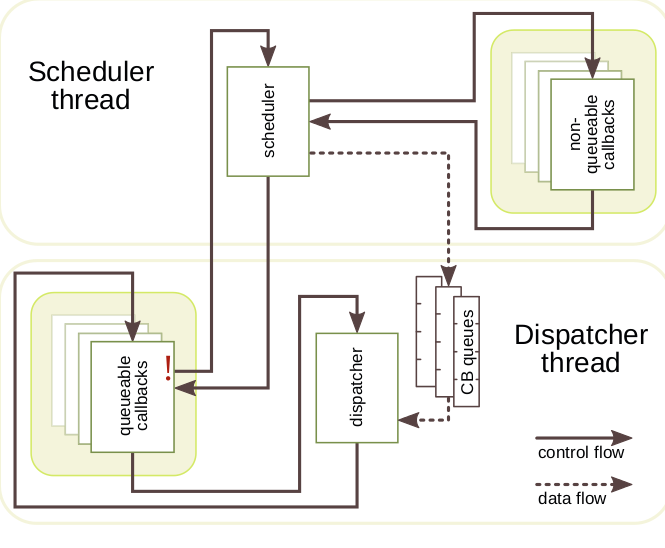
\includegraphics[width=250pt,height=150pt,scale=2]{Pics/event-handling.png}
\centering
\caption{Event-handling. The control and data flow is shown\cite{sharp2011event}}
\end{figure}

The types of callbacks can be seperated in two categories. Queueable and non-queueable. In the case of a non-queuable callback, the callback is executed immediately by the system, having the top priority of execution. A queueable callback, which is most common, will be put on an execution queue along with other queueable callbacks. In the case that the queue empties, no callbacks will be executed. It will continue executing callbacks when another event occurs at some point\cite{sharp2011event}\cite{rast2012managing}. 
	
\subsection{Notable work using the SpiNNaker architecture}
Most of the notable work done in SpiNNaker machines is simulation of neurons. Various simulations would use different kinds of neurons\cite{rast2012event}\cite{rast2011event}\cite{davies2011maintaining}\cite{jin2010algorithm}. One of the most interesting examples is simulating the neurons of the retina, so as to make it possible for a robot to calculate its place\cite{davies2010interfacing}. Another one would be simulating thousands of spiking neurons using four million synapses\cite{sharp2012power}. Finally, another intriguing application is teaching the neurons temporal sequences  of discrete symbols by using a test data set, thus making fast and accurate predictions of new sequences\cite{bose2005spiking}.

\subsection{Conjugate Gradient Method}
The Conjugate Gradient Method is an algorithm for the numerical solution of systems of linear eqations of the type Ax=b, those whose matrix is symmetric and positive definite. 

A \emph{symmetric} matrix is a matrix which is equal to its transpose. If A is a symmetric matrix then $A=A^T$. The entries of the matrix are symmetric with respect to the main diagonal, so if an element of the matrix A is a, then $a_{ij}=a_{ji}$. 

A \emph{positive definite} matrix M is a matrix which when multipled by any non-zero vector z and its transpose $z^T$, is always positive. In short the relationship that needs to be satisfied is $zMz^T$>0

It is an iterative method, which means it can be applied to sparse systems. A \emph{sparse matrix} is a matrix which is populated primirily with zeros. Its opposite would be a \emph{dense matrix}. The algorithm was developed by Magnus Hestenes and Eduard Stiefel and can be used to solve optimization problems\cite{press2007numerical}.
\subsubsection{The quadratic form}
In order to explain why the Conjugate Gradient Method can solve problems whose matrix can only be positive-definite and symmetric an explanation of the quadratic form needs to be presented. The following explanation will also outline the reason why this algorithm is used in optimisation problems too.
\begin{center}
\begin{equation}
f(x)=\frac{1}{2}x^TAx-b^T+c
\end{equation}
\end{center}

The gradient $\nabla f(x)$ of the quadratic form is a vector field that points in the direction of the greatest increase of $f(x)$. If we were to take into account the i$^{th}$ component of $\nabla f$, then.
\begin{equation}
\begin{split}
f(x+\psi e_i)= \frac{1}{2} (x+\psi e_i)^TA(x+\psi e_i)-b^T(x+\psi e_i)+c\\
= \frac{1}{2} (x^TAx+\psi e^T_iAx +x^TA\psi e_i)-b^T(x+\psi e_i)+c
\end{split}
\end{equation}
Note that e$_i$ is the error affiliated with taking the i$^{th}$ component of $\nabla f$. Now from the definition of a derivative $f(x)$=$\frac{f(a+h)-f(a)}{h}$ and (2) we have.
\begin{equation}
\frac{f(x+\psi e_i)-f(x)}{\psi}=\frac{\frac{1}{2}(\psi e^T_iAx+x^TA\psi e_i)-\psi e^T_ib}{\psi}
\end{equation}
(3) is the same as the i$^{th}$ component of $\frac{1}{2}$(Ax+A$^T$x)-b
So we have
\begin{equation}
\nabla f =\frac{1}{2}A^Tx+\frac{1}{2}Ax-b
\end{equation}
But if A is symmetric, then it is obvious that we have $Ax=b$ at the minimum of $f$. In addition if A is positive negative then $f$ is concave up.
\subsubsection{Conjugate Gradients}
As mentioned before the matrix A must be symmetric and positive definite for the Conjugate Gradient Method to work. Given a quadratic function 
as defined in (1), then it turns out that $-\nabla f=b-Ax=r$.

The CGM, as well as most optimization methods(for example the method of the Steepest Descent\cite{rosenbloom1956method}), look towards a specific direction everytime they are to move to a correct position and try to look for the best step given their gradient and direction
\begin{equation}
x_{k+1} = x_k + \alpha p_k
\end{equation}
Given (5), $\alpha$ can be deduced from the fact that $e_{k+1}$(the error vector of each iteration) must be orthogonal to p$_k$,  which also means that p$_k$ will never be met again as the solution progresses. Using this we can dedcuce
\begin{equation}
\begin{split}
p^T_ke_{k+1}=0\\
p^T_k(e_k+\alpha p_k)=0\\
\alpha = -\frac{p^T_ke_k}{p^T_kp_k}
\end{split}
\end{equation}

The equation at (6) however is not solvable. The value of $e_k$ is needed in each iteration, which is not computable at that time. To help with that the search directions in each iteration($p_k$) is defined as A-orthogonal in respect to the matrix A, instead of just orthogonal. The definition of A-orthogonal vectors is, given a matrix A, then:
\begin{equation}
p^T_kAp_k=0
\end{equation}
Given (7), $e_{k+1}$ and $p_k$ must be A-orthogonal. If we wish to find the optimal value for $\alpha$,then the gradient must be set to 0. This leads to the following equation.
\begin{equation}
0=\frac{d}{d\alpha}f(x_{k+1})=\nabla f(x_{k+1})^T\frac{d}{d\alpha}x_{k+1} = -r^T_{k+1}\frac{d}{d\alpha}(x_k + \alpha p_k) = -r^T_{k+1}p_k=p^T_kAe_{k+1}
\end{equation}
From (6),(7) the equation for $\alpha$ when $e_k$ and $p_k$ are A-orthogonal is
\begin{equation}
\begin{split}
\alpha =-\frac{p^T_kAe_k}{p^T_kAp_k}\\
=\frac{p^T_kr_k}{p^T_kAp_k}
\end{split}
\end{equation}

Another important equation that comes from analysing the error term is
\begin{equation}
p^T_kr_k=u^T_kr_k
\end{equation}

In (10) $u^T_k$ are u vectors that span the vector subspace of the vector field of $p_k$. They are also orthogonal to $r_k$ and $u_{k+1}$ is also orthogonal to all the previous $u$ vectors.

Using (9) and (10) we are able to reach a more accurate value for $\alpha$
\begin{equation}
\alpha = \frac{r^T_kr_k}{p^T_kAp_k}
\end{equation}

Using (9) and (10) and a Gram-Schmidt conjugation we are able to reach and a value for $\beta$
\begin{equation}
\beta = \frac{r^T_{k+1}r_{k+1}}{r^T_kr_k}
\end{equation}
\newpage\cite{rast2012managing}
\subsubsection{The algorithm}
Combining the optimal value of $\alpha$(8) and $\beta$(9) and a good step direction for p$_k$ the Conjugate Gradient Method is formed as follows
\\
\begin{algorithmic}
\STATE r$_0$=b-Ax$_0$
\STATE p$_0$=r$_0$
\STATE k=0
\FOR{k to 1000000}
\STATE $\alpha_k=\frac{r_k ^T*r_k}{p_k ^T*A*p_k}$
\STATE x$_{k+1}$=x$_k$+$\alpha_k$*p$_k$
\STATE r$_{k+1}$=r$_k$-$\alpha_k$*p$_k$*A
\IF{r$_{k+1}^T$*r$_{k+1}$ is small enough}
\STATE break
\ENDIF
\STATE $\beta_k=\frac{r_{k+1} ^T*r_{k+1}}{r_k ^T*r_k}$
\STATE p$_{k+1}$=r$_{k+1}$+$\beta_k$*p$_k$
\STATE k=k+1
\ENDFOR
\end{algorithmic}
\vspace{20pt}
Some notes that can be made about this algorithm are that the axis is defined by the eigenvectors of A and that the algorithm takes a conjugate step closest to $r$. Finally, the algorithm guarantees convergeance in at most n steps.\cite{press2007numerical}\cite{shewchuk1994introduction}\cite{cgm2009lec}

Ofcourse there is an error that exists in every step, as mentioned before, but it is minimized in each iteration. The error function would be:
\begin{equation}
\begin{vmatrix}
e_k
\end{vmatrix}
\leq 2(\frac{\sqrt{\kappa}-1}{\sqrt{\kappa}+1})^k
\begin{vmatrix}
e_0
\end{vmatrix}_A
\end{equation}

In Equation 9 $\kappa$ is the condition number.

Another interesting applicatoin of the Conjugate Gradient Method is that you can apply precondition on it in order to find the solution faster. However, preconditioning is outside of the scope of this project, since it adds a lot more calculation and would need a less general solution.

In general, the time complexity of the CGM is $\sqrt{n}$, where n is the size of the input matrix. Performing this algorithm sequentially would make the matrix-vector multiplication finish in $O(N^2)$ steps and the inner products in $O(N)$ steps.
\subsubsection{Parallel solutions of the CGM}

Some parallel implementations of the CGM use blocks(parts) of the input vectors and matrix and assign them carefully to specific cores, thus letting each core produce output that will be used in the next iteration. These kinds of solutions work better with vector processors of high processing capabilities, since they are customised for the algorithm's specification. Depending on how many processors a machine has, parts of the algorithm can continue being sliced to blocks, until the optimal implementation is reached\cite{o1987parallel}.

Some other parallel implementations try to use more specific preconditionings to achieve faster results, but again for the parallel part, they split the input into blocks to distribute it to various cores\cite{adams1985m}\cite{adams1983m}. 

One of the most interesting implementations of the CGM, suggests an improved algorithm named ICGS(Improved Conjugate Gradient Squared), which is based in another already altered version of the CGM\cite{maheswaran1999mcgs}. This implementation computes all vector-matrix  multiplications and inner products concurrently, for each iteration. The communication time between these operations and vector updates has been organised efficiently, so that global communication drops significantly, thus dropping the run time of the algorithm as well\cite{yang2001improved}.

Finally, there are many recent implementations which have used GPU's in order to solve the Conjugate Gradient Method efficiently. These techniques use CUDA as their main tool and various other techniques to accomplish their goal with some very good results. Solutions in different GPU models exist but that just enhances the generality of the solution using a GPU architecture. Generally though,as is for most parallel implementations of the CGM, the most used technique is reducing the time it takes to compute the matrix-vector multiplication and inner products, thus reducing the time of the algorithm overall\cite{galiano2012gpu}\cite{wozniak2010parallel}.
\section{Design}
As it was stated in the introduction the purpose of this project was to significantly reduce the time that the CGM takes to run, by reducing the time complexity of its most expensive computations. These computations were matrix-vector multplication and inner-products. In this section the basic communication, the matrix-vector multiplication and the flow of the program is considered. In addition to that the contents of the Target Tables are shown, along with the way the event handlers decide what operation to do, namely the Operation Codes. The section finishes, by discussing some of the design choices that were made. 

Throughout this section, an element of the matrix,vectors and constants in the algorithm which will be placed into a core is going to be refferred to as a \emph{node}. This way the algorithm will be viewed easier as a graph in the SpiNNaker system, which might help with the visualisation of the problem.

\subsection{Basic communication}
Using the massive parallelism that the SpiNNaker architecture provides with over a million cores, it was a clear step that each element of the input matrix(A) and vectors(b,r) would be put into a different node. 
\begin{figure}[h!]
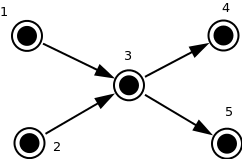
\includegraphics[width=250pt,height=150pt,scale=2]{Pics/basic.png}
\centering
\caption{Basic communication between nodes.}
\end{figure}
Considering that choice, it is easy to see that each node would need to receive and send spikes to a number of other nodes at any given time, in the same fashion that Figure 6 shows. In Figure 6 node 3 receives packets from nodes 1 and 2 and after some manipulation of the incoming data it sends its results to nodes 4,5. 

If this model is to be used each computation would be completed atomically and if only one computation is needed every time then the complexity at each core would be $O(1)$.
\subsection{Matrix-Vector Multiplication}
Using the above model a matrix-vector multiplication would look like Figure 7. 
\begin{figure}[h!]
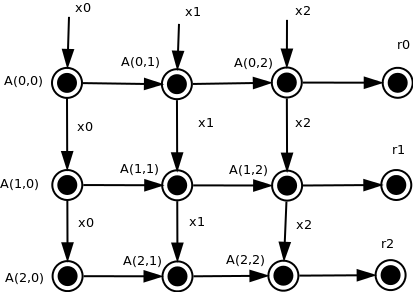
\includegraphics[width=250pt,height=150pt,scale=2]{Pics/mat0mult.png}
\centering
\caption{Matrix-vector multiplicatio for A*x.\cite{basicinterim}}
\end{figure}

In Figure 7 the first matrix-vector multiplication of the algorithm is used($Ax=r$) as an examplee to display the general overview of this operation. In this figure the example of a 3x3 $A$ matix and 3x1 vectors is used for simplicity. Also assume that the respective element of the vector $b$ is already there, waiting to complete the calculation for $r$, once the multiplication is over. To do the calculation, the $x$-nodes send a packet with their value to the respective $A$-nodes, where the multiplication part is completed. The $A$ nodes know which packets they should receive. because the connections between nodes have been provided externally by the user. The packets from $x$ reach the $A$ nodes because they are multicast. The column of the element in the matrix is considered to identify which $x$ nodes should be received by the $A$-nodes. The figure shows without precision that $A$-nodes send their value to the next $A$-node in the column. This has been done for means of clarity, but what the graph means to show is the $x$ nodes sending their value down the line. The same applies for when a $A$-node, after having completed the multiplication, sends the result to its respective $r$-node. Each time a packet arrives in the $r$-node an addition occurs, so as to complete the additive part of the multiplication. 

In Figure 7 the node $x_0$ sends its value to the $A$ nodes with column 0($A_{0,0} A_{1,0} A_{2,0}$). Once the muliplication in each of these nodes is completed, the result is sent to the $r_0$ node. The same holds for the other two sets of $A$ nodes and their respective $r$ node. 

Given the figure above, it is clear that the multiplication in each $A$-node is done in $O(1)$. The same applies for the addition in the $r$-nodes, since there is some delay from the time the packet is sent and the tme it arrives. Considering the communication tree built and discussed in section 2.3.2, the overall time-complexity for a matrix-vector multiplication to occur is $O(1)+log_2(N)+O(1)$. However, this is an optimal time-complexity that requires only one computation in each node. In practice as it will be explained later, the complexity is larger.
\subsection{Program Flow}
Given what has been discussed so far consider the following figure.
\begin{figure}[h!]
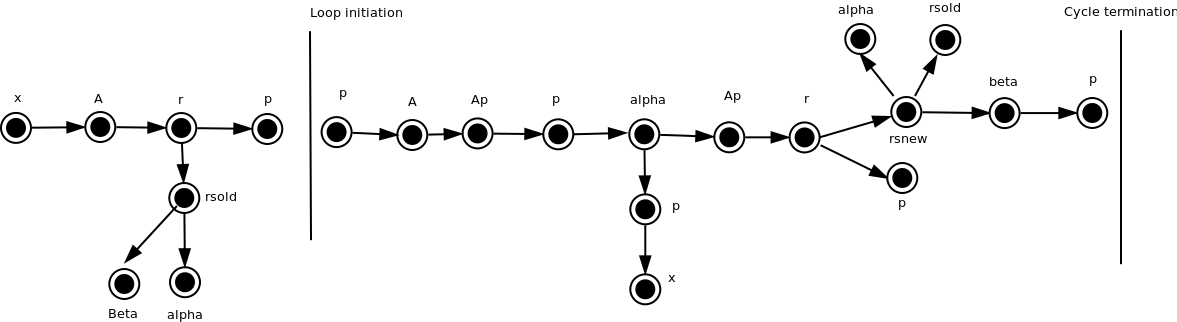
\includegraphics[width=500pt,height=150pt,scale=1]{Pics/program_flow.png}
\centering
\caption{The program flow in class diagram.}
\end{figure}
Figure 8 demonstrates the program flow of the CGM through the SpiNNaker machine. Each node in the figure represents a number of nodes during run time. If the example from the previous section is continued(a 3x3 matrix) the $x$ node in the beginning of Figure 8 represents 3 actual nodes. The $A$ node in Figure 8, represents $n^2$ nodes, since it has $nxn$ dimensions.

In addition to the input nodes $x,A,b$ it is viewable that there are some more nodes that exist throughout the algorithm. These nodes are helper nodes, without whom the algorithm would not be solvable in this context. A set of nodes that is not found in the CGM algorithm explained previously are Ap nodes. These nodes are used to save the result of the $A*p$ computation and help towards running the algorithm.

Some constant nodes that can be found in Figure 8 are also noteworthy. These are $\alpha$(alpha in Figure 8),$\beta$,(beta in Figure 8),$rsold$ and $rsnew$. These nodes were used to compute and save constant values that are needed for the computation of the algorithm. The constant $\alpha$ and $\beta$ can be found in the original algorithm which means their existence is clear, but this is not the case for $rsold$ and $rsnew$. These constants are used to save the result of the inner product $r^Tr$ in each iteration. Since both $r_k$ and $r_{k+1}$ are needed in each computation, two variables are used to save their respective result.

Notice that the program flow is quite sequential in the way it executes, so as to avoid bad timing, which will result in wrong computations. Even though the flow seems sequential, the algorithm runs in parallel for each calculation. Some cases where the program flow seems to be more parallel is when rsold and rsnew send to many different kinds of nodes at once.

Another point of interest would be that there is not a node of type $b$ in Figure 8, which from the definition of the algorithm is seemignly an input node. It was decided that it would be best to place the $b$ node values immediately to the $r$ nodes, so as to speedup the calculation, save space and cores, and reduce complexity. This step is allowed by the calculation, since $r$ nodes at the beginning of the algorithm are initialised to 0.

Finally, it should also be mentioned that after the first iteration of the algorithm whatever operation exists before the loop initiation is not needed.
\subsection{Target Table}
As mentioned in the Background section each node in the system has a Target Table entry, which helps each node complete various computations by reading its contents. The Target Table entry is customizable for each application. For the Conjugate Gradient Method the Target Table entry is as follows.
\begin{itemize}
\item unsigned Kd
\item vector<queue<unsigned>> OpCodes
\item char Name
\item usigned YD
\item unsigned X
\item unsigned Y
\item float Value
\item float Temp
\item unsigned counter
\item unsigned V
\end{itemize}

The Kd identifies the key of the node, which is individual to each node in the system. 

The Name identifies the type of which the node belongs to. The YD variable is the Y dimension of the element. For example, if the algorithm could take as input a 4x3 matrix, then the Y dimension would be 4 and the X dimension 3. However, in the CGM the matrixes are symmetric and the vectors have as an X dimension 1, so XD would be redundant to add in the table. 

The X and Y variables are there to identify the position of the node in the matrix or vector that it belongs to. 

The floats Value,Temp and unsigned counter are the original values of Value,Temp and counter, which are mainly there to show that these kinds of variables exist and are used for each node. Their position in the table is not vital, since their values cannot be changed trhoughout the program in the Target Table. 

Finally, there is the variable V, which is used to identify the position of the variables Value,Temp,counter and OpCodes in each core depending on the node that it belongs.
\subsubsection{OpCodes}
OpCodes in this context stands for operation codes, as in what operation needs to be done at any point in a specific node. Throughout the algorithm different kinds of operations are done. Be it addition,multiplication, subtraction etc., different operations need to be completed at different points of the program. Thus an unsigned integer is used to identify these operations upon the arrival of a packet. So for example, 1 would be used to identify addition, 2 for multiplication etc. The operation would be specified after the node went through a series of cases in a switch statement that would be checked against the OpCode that the node specified.

If the program flow is looked thoroughly, it is apparent that some nodes need to do different computations at different points of the algorithm. For example, a $p$ node needs to either store the value of its respective $r$ node, or do a computation such as $\alpha *p$. These are two completely different operations that need to be accounted for. Given that the easy solution would be to use a vector to save all the operations that need to be done and after reading the first element of the vector and completing the respective operation , put it in the back of the vector, since CGM is an iterative algorithm and some computations need to be repeated.

However, just a vector would not work. Consider the following. Based on the general connectivity between nodes the $\alpha$ node can receive packets from both $r$-nodes and $p$-nodes. That means that just before the loop initiates on Figure 8, the $\alpha$ node will receive packets both from $r$-nodes and $p$ nodes. In addition to that, $r$ nodes send their values to $p$ nodes. There is a chance that packets from $p$ nodes will reach the $\alpha$ node sooner than $r$ nodes do. In the case of $p$ nodes arriving, the operation would be to do nothing, since that information is not needed at that point and in the case of $r$ nodes arriving to compute the inner product.  This sequence of events cannot be forseen and with just a vector to represent the OpCodes the wrong calculation is to be expected.

Thus the choice of a vector of queues was made. With this data structure, the index of the vector is selected to act as a key to find the type of the node that the packet came from. Each type of node has a distinguished offset in the source address that will make it identifiable to the vector. For example, nodes from the matrix A have an offset of 0. Once the offset is read by the vector, a queue will come up. The front integer of the queue will be the operation that needs to be carried out at that point for the packet that had just arrived. Afterwards, in the same fashion as with the vector, the front OpCoed of the queue will be placed in the back of the respective queue for the next iteration.

By using this data structure it is apparent that the time complexity at each core has increased, because more operations take place. However, using a vector of queues of unsigned integers does not increase the complexity dramatically. The operator for accessing a vector is $O(1)$. The same applies for each of the following actions: looking at the front value of the queue, popping it from the front of the queue and pushing it in the back of the queue. Considering this the time complexity at each core has a small increase totalling $O(4)$.
\subsection{Justification for Design Choices}
At this point a justification for some design decisions would be appropriate. 

The SpiNNaker architecture gives you the choice of having global variables that would be accessible by all nodes of the system. That feature would be usable considering constant values such as $\alpha$ and $\beta$. Instead nodes were selected to contain and compute these values. The reason for that was that better control over computation on certain constants was provided when using constant nodes. This is because there was certainty that the value would change only when it was supposed to(when a packet would arrive in that constant node), whether with a global value reading a wrong value was a possibility.

Another important design decision was the use of the vector of queues data structure. Given the iterative nature of the algorithm, following a model such as the one described has proved be very usable and simple and program. There existed an option of using a graph of nodes with multiple connections used, but that option was deemed too complicated, with the possibility of not even being implementable given the nature of this algorithm. However, it might have worked for other algorithms that do not require iterations to find solutions and did not involve many steps.
\section{Implementation}
In this section some implementation details are going to be outlined. More specifically a description of the simulators used, the process that the keys were generated. In addition, the iterations after the first one will be described as well as the general specification of the OpCodes for each node.
\subsection{Simulators//mb put it in testing}
To test the implementation of the program simulators of the SpiNNaker chip were used. These were supplied by the supervisor of this project and were written in the C++ language. 

The main development and testing of this algorithm was made in the first simulator. In that simulator the programmer had the ability to use STL(Standard Template Library), which helped towards abstracting the problem and leaving out some implementation details. It would also write out the binary files that the second simulator and the actual machine would use. The simulator however was configured to comply better with the specification of this project.

The second simulator was much less flexible towards using data structures, since it had to simulate much better the reaction of a SpiNNaker chip, when data and a program was loaded to it. It read the same binary files that the SpiNNaker machine would read for data and the event handlers written for it resembled the actual event handlers much more.

\subsection{Offset}
As mentioned in the Design section, the vector of queues of integers(OpCodes) uses a key to identify which kind of node a packet has arrived from. In order to generate the key 4 elements are used. These are
\begin{itemize}
\item X position of the chip in the mesh
\item Y position of the chip in the mesh
\item Core number
\item Offset which is the ID of the node in the core.
\end{itemize}
The offset for each element is allocated at the time that all keys are generated. A switch statement was used to distinguish the nodes by name and then alter the offset according to the name. 

Since each core can theoretically have more than one nodes allocated to it, redefining the offset might cause some problems. For example, if elements of the same type and offset are allocated to the same core then one of them might be ovewritten. 

However, if that practice is avoided then this problem will not occur. In addition to that, the solution to this problem has been designed so as to allocate one node of whatever type to only \emph{one} core, so as to achieve the highest speedup possible. Hence putting more than one elements to a core would not comply with the overall design of this project.
\subsection{Second Iteration}
As mentioned before, after the first iteration some operations must not be completed again, so as to not distrupt the completion of the algorithm. These operations are the ones that are left from the "Loop Initiation" line in Figure 7. To accomplish that a special callback(function) was written. This function would be called only once throughout the run time of the program once all remaining packets had arrived at the $p$ nodes(See last node in Figure 8). That function would issue commands to all the nodes in the system, making them remove at least one OpCode from one of the queues, based on the type of element it is. Again the name of the element was considered to make that decision.
\subsection{Input files}
In order to simulate and run a program an input file would have to be put on the first simulator, so as to process the data and write the binary files. Hence a file format was invented to comply with the specification of this project. An example of the input file is shown in Appendix(8.1). At the Values section, the elements of matrices, vectors and constant nodes are described. The names, dimensions inside the brackets and actual values are specified. The OpCodes for each type of element are also viewable. They are the integers next to the dimensions of each matrix/vector/consant. The first integer is the key and all the others are actual OpCodes. Different queues are seperated with a semicolon. In the Connections section, the connections between nodes are specified. The general layout for the OpCodes for any size matrix  is shown in Appendix 8.2.
\subsection{Implementation OpCodes}
As explained before, the SpiNNaker architecture does not support any libraries that would help form a queue data structure, which, as a step, is pivotal to the design analyzed previously. In addition to that, the contents of the binary files are read one at a time, so an STL queue would not be readable from them. Finally, SpiNNaker cannot read serialised data, so serialisation was not a valid option either.

Considering all the aforementioned parameters, it was decided that the vector of queues of unisgned integers, would be impemented using only an array. To successfully translate the vector of queues of integers data structure the following format was selected.

\begin{enumerate}
\item Number of queues.
\item Size of next queue.
\item Head
\item Tail
\item Key.
\item Data.
\end{enumerate}
The number of queues(1) would exist only once in each array, so as to know how many different queues exist. The information from 2-6 is the information that the array would need to simulate one queue. This information would be repeated in each array, depending on how many queues existed. The size and the key would appear only once in each simulated queue, whereas the data consists of the actual OpCodes that each node would look into to execute the next operation. The Key is the index that the vector would look using the offset of the incoming packet. Finally, the Head and Tail would act as pointers to the first and the last element of the queue respectively, so as to execute queue like operations.

Given the above format, three functions were also implemented to do operations on that array and more precisely in the simulated queues in that array. These were front(),pop() and pushandpop(). Depending on the offset of the source key of the arrived packet the front() function would show the first integer on the simulated queue, pop() would remove the OpCode in the front position from the queue and pushandpop() would put the OpCode in the first position in the back of the queue. When using pop(), the OpCodes is not actually removed, but rather the tail is reduce, so as to not be able to access it again.
\subsection{Connections and OpCodes programs}
In addition to the implementation of the algorithm, two additional programs were constructed in order to create the input files quickly and without errors. 

A Connections C++ program was written to create the connections between nodes and add them in the Connections part of the input .mx file. For the connections between the matrix and the vectors, the rows and columns of the elements were taken into account. For the nodes containing constant values, the connections with other input nodes were more constant, but would also vary given the size of the input matrix and vectors. 

An OpCodes C++ program was written to produce  the operation codes for each node and also add it to the .mx input file. To create this program the general layout of OpCodes in Appendix 8.2 was used.

Combining these two programs, most of the input file is written automatically. All the user needs to do is insert the dimensions of the input vectors and matrix correctly and their corresponding values. These programs made the testing phase easier.
\section{Testing}
The testing phase of the algorithm took place in both of the simulators. This needed to be done because not only should the result of the algorithm had to be verified, but also because corruption of binary files is also a possibility that needed to be tested. In addition to that, the implementation queue needed to be tested.

The actual testing was made by using different kinds of matrices, with different values and different sizes. This was done to test whether the solution of the algorithm was scalable and robust. The results from the simulators were cross referenced with the results from a sequential implementation of the algorithm to check their validity. A couple of examples of the tests made and their results are shown in Appendix 8.3. More examples can be found in the Github repository where most implementation files are saved\cite{git_repo}.

All of the tests worked in both of the simulators successfully, while producing the correct and expected output. Throughout the testing phase there were no problems with corrupted binary files.
\section{Evaluation}
In general the design and implementation that has been proposed and tested throughout this project has been proven to be robust and scalable. Using the data structure of vector of queues provides a solution not only for the solution of the Conjugate Gradient Method, but also other algorithms that might be similar to this one. Using the proposed design, a programmer could implement other algorithms by sketching out a program flow similar to Figure 8, and then finding the connections between the nodes. In addition, using the proposed design offers the advanatge of few and understandable connections between nodes that can be easily produced using a simple program.

One disantvantage of the design is the additional complexity that it adds in each computation from $O(1)$ to $O(4)$. However this is not a dramatic increase and will not reduce the speedup dramatically. In addition, creating a customised vector of queues of integers using an array might prove to be complex if used for some other algorithms. However, if the design proposed in the Implementation section of this project is followed, then the task might prove to be easier.

One improvement that this project could have benefitted from is running the algorithm in a SpiNNaker chip to see if it would work in the actual machine as good as it would have in the simulators. Having tested that, by using the SpiNNaker chips, the practical speedup that the architecture provides could have been found and compared to the sequential implementation of the algorithm, as well as other parallel implementations. Unfortunately, the time available with a SpiNNaker board was limited and in addition to that there was a malfunction to the board.

In addition, more testing could have been carried in the simulators out throughout this project to make sure whether the algorithm could scale to matrices with very high dimensions i.e. a 400x400 sparse matrix. The tests that were carried out do indicate that a correct solution would have been produced, but doing the actual testing would improve upon the validity of the solution.

In the event handler it is visible that there are around 13 different operations that can be carried out by all the nodes. This number could be reduced from 13 to 11 or 10, by optimising some of the operations that each case does. During the implementation stage, a higher number of operations was chosen in order to test each operation's validity more atomically.

The hardest part of this project was coming up with an efficient way of doing operations in each node, while preserving a low time complexity in each computation and also producing the correct result. The vector of queues of integers that was selected to represent OpCodes, while using the Offset of each incoming packet's source address as a key to the OpCodes. One of the easier tasks of this project was the creation of the programs to automatically produce the OpCodes for each node and the connections between them.
\section{Conclusion}
In conclusion, this project achieved the goal that was outlined in the project brief by finding a solution to the algorithm using the SpiNNaker architecture. It took advantage of the massive parallelism that the architecture provides and was able to dramatically reduce the time complexity of the most expensive operations of the algorithm. The matrix-vector multimplication was reduced from $O(N^2)$ to $O(4) + log_2(N) + O(4)$ and the inner product from $O(N)$ to $O(4)$. 

\newpage
\bibliographystyle{plain}
\bibliography{ref.bib}
\cite{navaridas2009understanding}
\cite{sharp2012power}
\cite{davies2010interfacing}
\cite{sharp2011event}
\cite{gerstner2002spiking}
\cite{press2007numerical}
\cite{shewchuk1994introduction}
\cite{cgm2009lec}
\cite{o1987parallel}
\cite{adams1985m}
\cite{maheswaran1999mcgs}
\cite{yang2001improved}
\cite{adams1983m}
\cite{galiano2012gpu}
\cite{wozniak2010parallel}
\cite{hestenes1952methods}
\cite{rosenbloom1956method}
\cite{furber2007neural}
\cite{spinnweb}
\cite{khan2008spinnaker}
\cite{docfile}
\cite{plana2007gals}
\cite{furber2012overview}
\cite{bose2005spiking}
\cite{jefflec}
\cite{basicinterim}
\cite{rast2012managing}
\cite{rast2012event}
\cite{davies2011maintaining}
\cite{jin2010algorithm}
\cite{git_repo}
\section{Appendix}
\subsection{Example Input file}
BEGIN VALUES\\
MX1[2,2] 1/1;4/1/0/0\\
4.0 1.0\\
1.0 3.0\\
X[2] 16/3;4/0/0/11\\
2.0 1.0\\
R[2] 0/2/0/0/0;5/0/10\\
1.0 2.0\\
P[2] 3/4/14;5/1/0;7/1;9/15\\
0.0 0.0\\
A[2] 0/0/0/6/6;7/1\\
0.0 0.0\\
RO[1] 3/5/0/0;6/7\\
0.0\\
N[1] 3/0/0/5\\
0.0\\
L[1] 2/7;4/0/0/8/8/0/0;6/7\\
0.0\\
CH[1] 6/13\\
0.0\\
B[1] 2/7;6/12\\
0.0\\
END VALUES\\
BEGIN OVERLAYS\\
END OVERLAYS\\
BEGIN CONNECTIONS\\
X[0]>MX1[0,0] MX1[1,0]\\
X[1]>MX1[0,1] MX1[1,1]\\
MX1[0,0]>R[0] A[0]\\
MX1[0,1]>R[0] A[0]\\
MX1[1,0]>R[1] A[1]\\
MX1[1,1]>R[1] A[1]\\
R[0]>P[0] RO[0] N[0]\\
R[1]>P[1] RO[0] N[1]\\
RO[0]>L[0] B[0]\\
P[0]>MX1[0,0] MX1[1,0] X[0] L[0]\\
P[1]>MX1[0,1] MX1[1,1] X[1] L[0]\\
A[0]>R[0] P[0]\\
A[1]>R[1] P[1]\\
L[0]>A[0] A[1] P[0] P[1]\\
N[0]>B[0] RO[1] CH[1] L[1]\\
B[0]>P[0] P[1]\\
END CONNECTIONS\\
\subsection{Outline of OpCodes}
n is the YD dimension of the MX1 matrix. When you see nx, it means n x's must be put there. For example if YD=2 and x=0 the OpCodes would actually be .../0/0/....
MX1->1/1;4/1/0/0\\
X->4/0/0/11;16/3\\
R->0/2/n0/0;5/0/10\\
P->3/4/14;5/1/0;7/1;9/15\\
A->0/n0/n6;7/1\\
RO->3/5/n0;6/7\\
N->3/n0/5\\
L->2/7;4/n0/n8/n0;6/7\\
CH->6;13\\
B->2/7;6/12\\
\subsection{Test examples}
A test with a 3x3 input matrix\\
BEGIN VALUES\\
MX1[3,3] 1/1;4/1/0/0\\
2.0 -1.0 0.0\\
-1.0 2.0 -1.0\\
0.0 -1.0 2.0\\
X[3] 4/0/0/11;16/3\\
5.0 7.0 8.0\\
R[3] 0/2/0/0/0/0;5/0/10\\
4.0 -8.0 1.0\\
P[3] 3/4/14;5/1/0;7/1;9/15\\
0.0 0.0 0.0\\
A[3] 0/0/0/0/6/6/6;7/1\\
0.0 0.0 0.0\\
RO[1] 3/5/0/0/0;6/7\\
0.0\\
N[1] 3/0/0/0/5\\
0.0\\
L[1] 2/7;4/0/0/0/8/8/8/0/0/0;6/7\\
0.0\\
CH[1] 6/13\\
0.0\\
B[1] 2/7;6/12\\
0.0\\
END VALUES\\
BEGIN OVERLAYS\\
END OVERLAYS\\
BEGIN CONNECTIONS\\
X[0]>MX1[0,0] MX1[1,0] MX1[2,0]\\
X[1]>MX1[0,1] MX1[1,1] MX1[2,1]\\
X[2]>MX1[0,2] MX1[1,2] MX1[2,2]\\
MX1[0,0]>R[0] A[0]\\
MX1[0,1]>R[0] A[0]\\
MX1[0,2]>R[0] A[0]\\
MX1[1,0]>R[1] A[1]\\
MX1[1,1]>R[1] A[1]\\
MX1[1,2]>R[1] A[1]\\
MX1[2,0]>R[2] A[2]\\
MX1[2,1]>R[2] A[2]\\
MX1[2,2]>R[2] A[2]\\
R[0]>P[0] RO[0] N[0]\\
R[1]>P[1] RO[0] N[0]\\
R[2]>P[2] RO[0] N[0]\\
RO[0]>L[0] B[0]\\
P[0]>MX1[0,0] MX1[1,0] MX1[2,0] X[0] L[0]\\
P[1]>MX1[0,1] MX1[1,1] MX1[2,1] X[1] L[0]\\
P[2]>MX1[0,2] MX1[1,2] MX1[2,2] X[2] L[0]\\
A[0]>R[0] P[0]\\
A[1]>R[1] P[1]\\
A[2]>R[2] P[2]\\
L[0]>A[0] P[0] A[1] P[1] A[2] P[2]\\
N[0]>B[0] RO[1] CH[1] L[1]\\
B[0]>P[0] P[1] P[2]\\
END CONNECTIONS\\

Results is:

$x=\begin{bmatrix}
-0.75\\
-5.5\\
-2.25\\
\end{bmatrix}$
     
A test with a 5x5 input matrix\\
BEGIN VALUES\\
MX1[5,5] 1/1;4/1/0/0\\
1.0 2.0 3.0 4.0 5.0\\
2.0 7.0 -4.0 -7.0 0.0\\
3.0 -4.0 10.0 9.0 -6.0\\
4.0 -7.0 9.0 11.0 -2.0\\
5.0 0.0 -6.0 -2.0 6.0\\ inputs
X[5] 4/0/0/11;16/3\\
-1.0 7.0 9.0 0.0 6.0\\
R[5] 0/2/0/0/0/0/0/0;5/0/10\\
3.0 -2.0 0.0 -9.0 1.0\\
P[5] 3/4/14;5/1/0;7/1;9/15\\
0.0 0.0 0.0 0.0 0.0\\
A[5] 0/0/0/0/0/0/6/6/6/6/6;7/1\\
0.0 0.0 0.0 0.0 0.0\\
RO[1] 3/5/0/0/0/0/0;6/7\\
0.0\\
N[1] 3/0/0/0/0/0/5\\
0.0\\
L[1] 2/7;4/0/0/0/0/0/8/8/8/8/8/0/0/0/0/0;6/7\\
0.0\\
CH[1] 6/13\\
0.0\\
B[1] 2/7;6/12\\
0.0\\
END VALUES\\
BEGIN OVERLAYS\\
END OVERLAYS\\
BEGIN CONNECTIONS\\
X[0]>MX1[0,0] MX1[1,0] MX1[2,0] MX1[3,0] MX1[4,0]\\
X[1]>MX1[0,1] MX1[1,1] MX1[2,1] MX1[3,1] MX1[4,1]\\
X[2]>MX1[0,2] MX1[1,2] MX1[2,2] MX1[3,2] MX1[4,2]\\
X[3]>MX1[0,3] MX1[1,3] MX1[2,3] MX1[3,3] MX1[4,3]\\
X[4]>MX1[0,4] MX1[1,4] MX1[2,4] MX1[3,4] MX1[4,4]\\
MX1[0,0]>R[0] A[0]\\
MX1[0,1]>R[0] A[0]\\
MX1[0,2]>R[0] A[0]\\
MX1[0,3]>R[0] A[0]\\
MX1[0,4]>R[0] A[0]\\
MX1[1,0]>R[1] A[1]\\
MX1[1,1]>R[1] A[1]\\
MX1[1,2]>R[1] A[1]\\
MX1[1,3]>R[1] A[1]\\
MX1[1,4]>R[1] A[1]\\
MX1[2,0]>R[2] A[2]\\
MX1[2,1]>R[2] A[2]\\
MX1[2,2]>R[2] A[2]\\
MX1[2,3]>R[2] A[2]\\
MX1[2,4]>R[2] A[2]\\
MX1[3,0]>R[3] A[3]\\
MX1[3,1]>R[3] A[3]\\
MX1[3,2]>R[3] A[3]\\
MX1[3,3]>R[3] A[3]\\
MX1[3,4]>R[3] A[3]\\
MX1[4,0]>R[4] A[4]\\
MX1[4,1]>R[4] A[4]\\
MX1[4,2]>R[4] A[4]\\
MX1[4,3]>R[4] A[4]\\
MX1[4,4]>R[4] A[4]\\
R[0]>P[0] RO[0] N[0]\\
R[1]>P[1] RO[0] N[0]\\
R[2]>P[2] RO[0] N[0]\\
R[3]>P[3] RO[0] N[0]\\
R[4]>P[4] RO[0] N[0]\\
RO[0]>L[0] B[0]\\
P[0]>MX1[0,0] MX1[1,0] MX1[2,0] MX1[3,0] MX1[4,0] X[0] L[0]\\
P[1]>MX1[0,1] MX1[1,1] MX1[2,1] MX1[3,1] MX1[4,1] X[1] L[0]\\
P[2]>MX1[0,2] MX1[1,2] MX1[2,2] MX1[3,2] MX1[4,2] X[2] L[0]\\
P[3]>MX1[0,3] MX1[1,3] MX1[2,3] MX1[3,3] MX1[4,3] X[3] L[0]\\
P[4]>MX1[0,4] MX1[1,4] MX1[2,4] MX1[3,4] MX1[4,4] X[4] L[0]\\
A[0]>R[0] P[0]\\
A[1]>R[1] P[1]\\
A[2]>R[2] P[2]\\
A[3]>R[3] P[3]\\
A[4]>R[4] P[4]\\
L[0]>A[0] P[0] A[1] P[1] A[2] P[2] A[3] P[3] A[4] P[4]\\
N[0]>B[0] RO[1] CH[1] L[1]\\
B[0]>P[0] P[1] P[2] P[3] P[4]\\
END CONNECTIONS\\

Result is:
$x=\begin{bmatrix}
-2.99911\\
9.6637\\
-16.4183\\
18.4744\\
-7.59421
\end{bmatrix}$

\subsection{Project Brief}
\newpage
\subsection{Gantt Charts}
To find better resolution pictures of the gantt chart see:\url{https://github.com/Alex-Oiko/3rd-Year-Project/tree/master/Deliverables/Final_Report/Gantt_Charts} \cite{git_repo}
\topmargin=0pt
\voffset=0pt
\begin{figure}[h!]
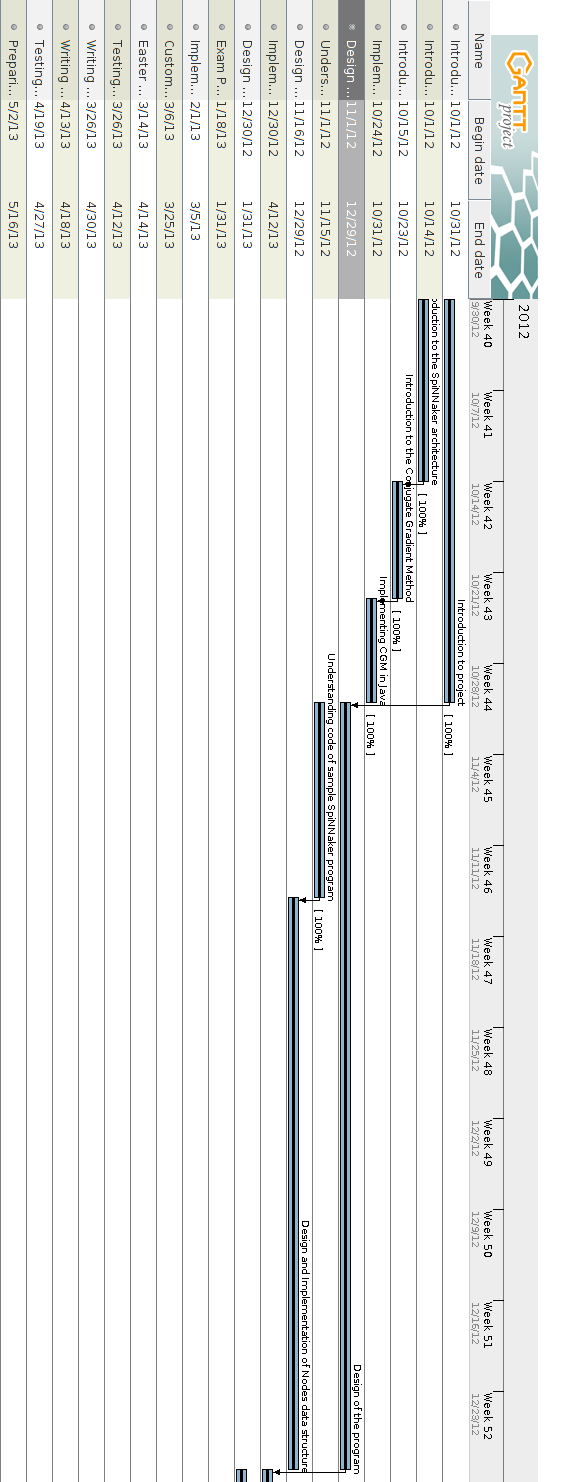
\includegraphics[scale=0.4]{Gantt_Charts/Final_Gantt1.png}
\centering
\end{figure}
\topmargin=0pt
\voffset=0pt
\begin{figure}[h!]
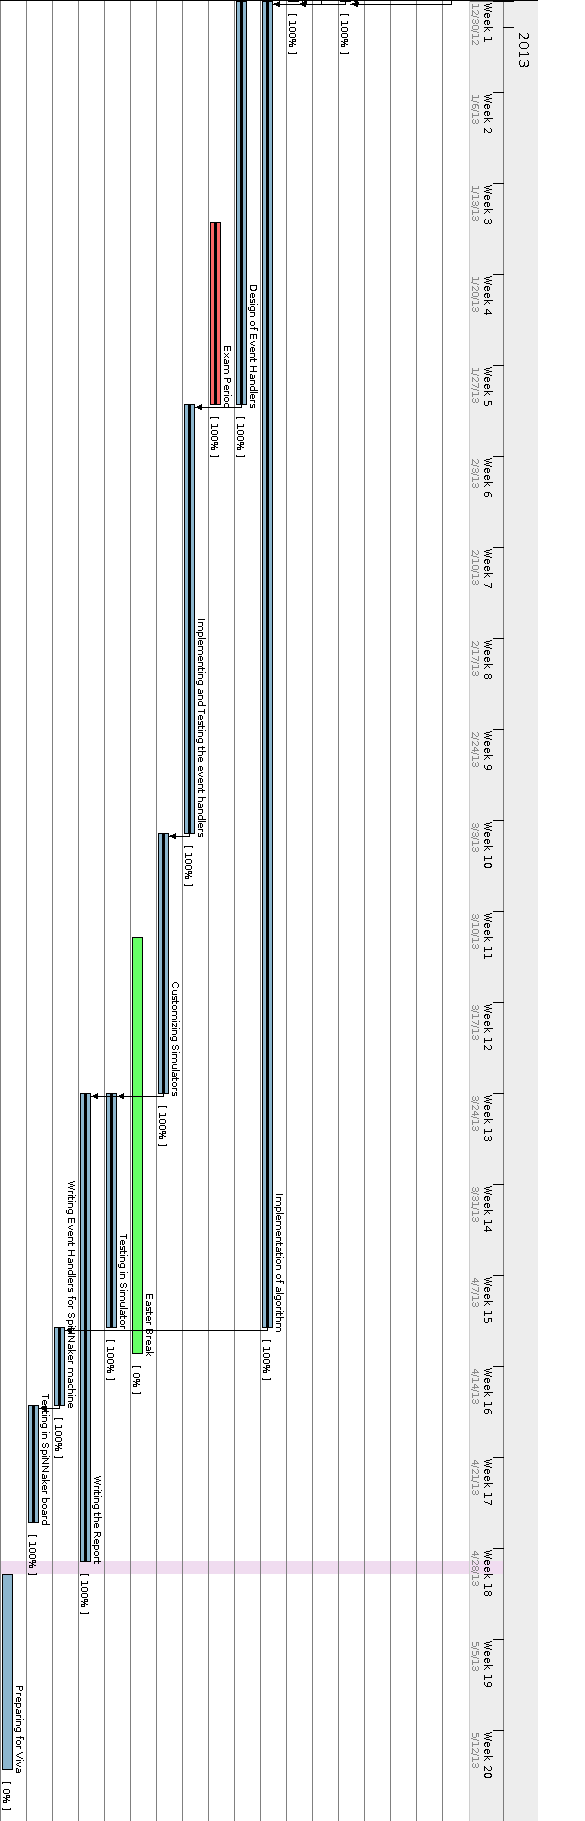
\includegraphics[scale=0.4]{Gantt_Charts/Final_Gantt2.png}
\centering
\end{figure}
\end{document}